\section{Zielsetzung}
\label{sec:Zielsetzung}
In diesem Versuch soll das Geiger-Müller-Zählrohr genauer untersucht werden. Es wird eine Charakteristik aufgenommen, mit der die Qualität des Zählrohr begutachtet wird.
Die Totzeit des Zählrohrs wird einmal mit einem Oszilloskop und einmal mit der Zwei-Quellen-Methode bestimmt. 
Aus dem mittleren Zählrohrstrom wird anschließend noch die Ladungsmenge pro einfallendem Teilchen berechnet.
\section{Theorie}
\label{sec:Theorie}
Das Geiger-Müller-Zählrohr hat einen zylinderförmigen Stahlmantel mit einem Draht in der Mitte, siehe \autoref{fig:aufbau_zählrohr}.
Es wird eine Spannung zwischen dem Mantel und den Draht angelegt, sodass sich im Inneren des Zählrohrs ein radialsymmetrisches elektrisches Feld mit der Feldstärke
\begin{equation*}
    E(r) = \frac{U}{r \cdot \log(\frac{r_{\text{k}}}{r_{\text{a}}})}
\end{equation*}
ausbildet.
Das Zählrohr ist gefüllt mit einem Gasgemisch.
An der Stirnseite des Zählrohres befindet sich eine Mylar-Folie, welche es den geladenen Teilchen einfacher macht in das Zählraumvolumes einzudringen und somit registriert werden können.
Die Folie ist wegen des Unterdruck im Zählrohr, wie in \autoref{fig:aufbau_zählrohr} zu sehen ist, nach innen gewölbt.
\begin{figure}
    \centering
    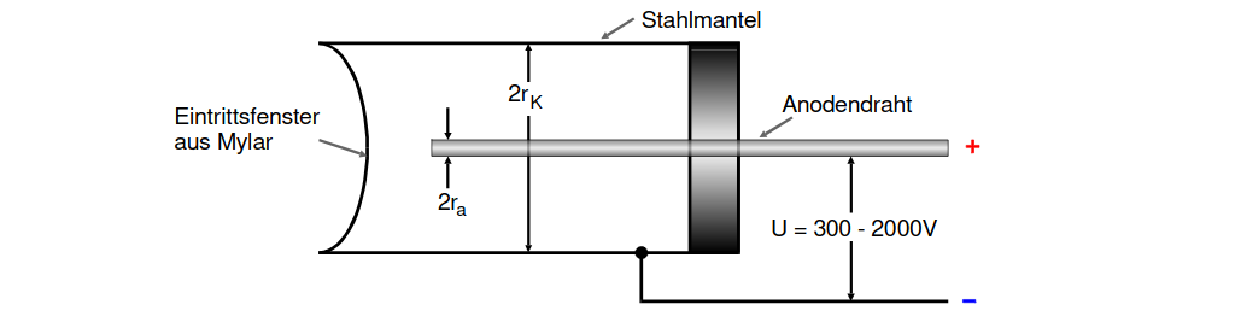
\includegraphics[width=\textwidth]{content/aufbau_zahlrohr.pdf}
    \caption{Querschnitt durch ein Endfenster-Zählrohr.\cite{anleitung}}
    \label{fig:aufbau_zählrohr}
\end{figure}
Wir ein geladenes Teilchen von dem Zählrohr absorbiert, bewegt es sich durch das Zählraumvolumen bis seine Energie durch Ionisationsakte aufgebraucht ist.
Dieser Primärionisation folgenden Ereignisse hängen von der angelegten Zählrohrspannung $U$ ab.
In der \autoref{fig:bereiche} ist die Anzahl der Elektronen-Ionenpaare für ein $\alpha$-Teilchen und ein $\beta$-Teilchen gegen die Spannung $U$ aufgetragen.
Es sind verschiedene Bereiche eingeteilt, die im folgenden diskutiert werden.
\begin{figure}
    \centering
    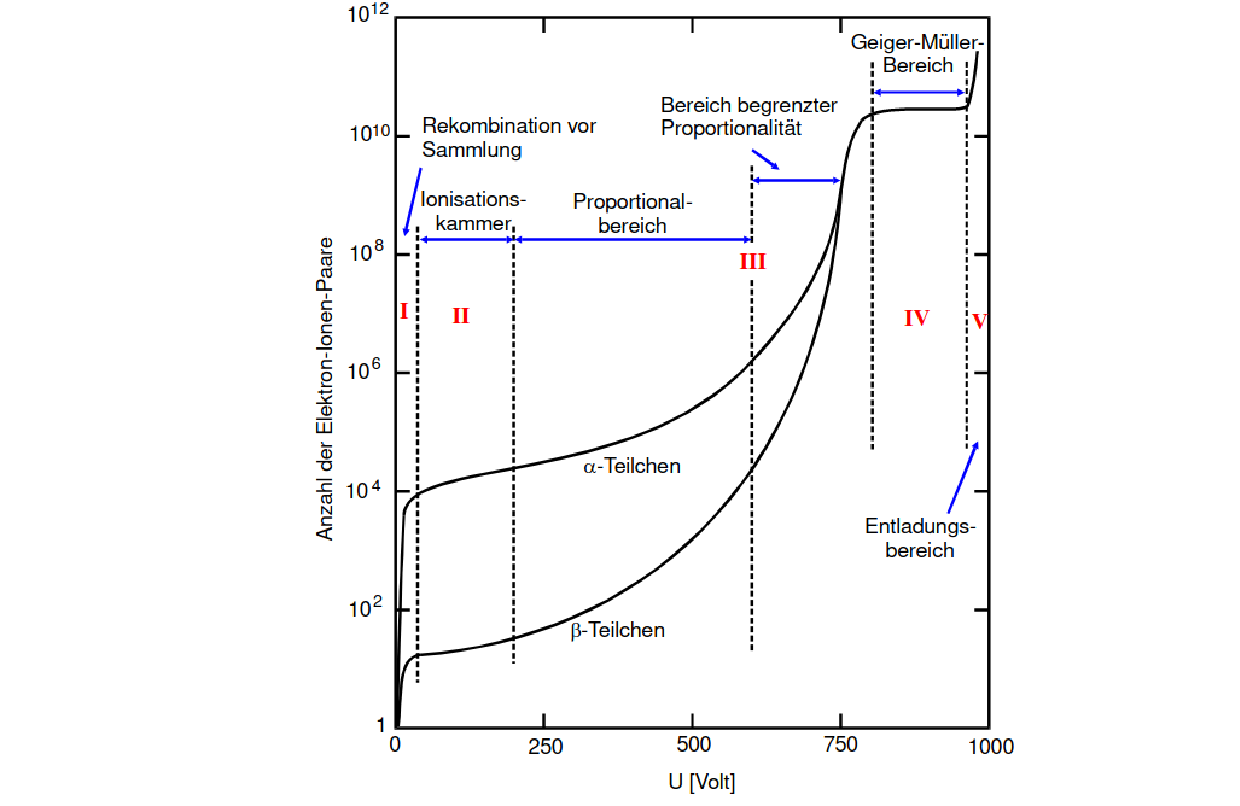
\includegraphics[width=\textwidth]{content/bereiche.pdf}
    \caption{Anzahl der erzeugten Elektron-Ionenpaare als Funktion der Spannung bei einem Proportionalzählrohr. \cite{anleitung}}
    \label{fig:bereiche}
\end{figure}
Bei einer geringen Spannung $U$ ist das elektrische Feld nicht groß genug, es gibt viele Rekombinationen und nur wenige der erzeugten Elektronen erreichen den Draht.\\
Dies enspricht dem Bereich I in der \autoref{fig:bereiche}.\\
In dem Bereich II ist die elektrische Feldstärke höher, sodass die Rekombinationswahrscheinlichkeit abfällt. 
Es bildet sich ein kontinuierlicher Ionisationsstrom zwischen Mantel und Draht aus, welcher proportional zur Energie und Intensität der einfallenden Strahlung ist. 
Ein so arbeitendes Gerät wird auch Ionisationskammer genannt und ist nur bei hohen Strahlungsintensitäten einsetzbar.\\
Nach weiterem Erhöhen der Spannung wird die Feldstärke des elektrischen Feldes so hoch, dass die ausgelösten Elektronen so stark beschleunigt werden. 
Die Elektronen haben schließlich eine genügend große Energie, sodass sie durch Stoßionisation wiederum selber Ionisieren können.
Diese schnell ansteigende Anzahl an Elektronen wird Townsend-Lawine genannt. 
Die Ladung, die für jedes einfallende Teilchen am Draht ankommt, kann nun als Ladungimpuls gemessen werden, der proportional zur Energie des einfallenden Teilchens ist.
Daher nennt sich ein in diesem Bereich III arbeitendes Gerät Proportionalzählrohr.\\
In dem Bereich IV in \autoref{fig:bereiche} liegt der hauptsächliche Arbeitsbereich des Geiger-Müller-Zählrohrs. 
In der Primärionisation entstehen UV-Photonen, die sich auch senkrecht zu den Feldlinien ausbreiten können, sodass im gesamten Zählraumvolumen Ladungslawinen entstehen.
Da die Ladungsmenge $Q$ nun vom Zählraumvolumen und der Höhe der Betriebsspannung abhängt, gibt es keine Abhängigkeit von dem Primärionisation und es kann keine Energiemessung druchgeführt werden.
Deswegen ist der Beginn des Auslösebereiches in der \autoref{fig:bereiche} dort, wo die Kurven der einzelnen Teilchen zusammenkommen.\\
Der letzte Bereich in der \autoref{fig:bereiche} ist der Bereich der Dauerentladung.
Die Feldstärke ist dann so groß, dass es zu einer andauernden Entladung kommt.
Es fließt ein sehr großer Strom, dass das Zählrohr zerstört werden kann.\\
\\
\begin{figure}
    \centering
    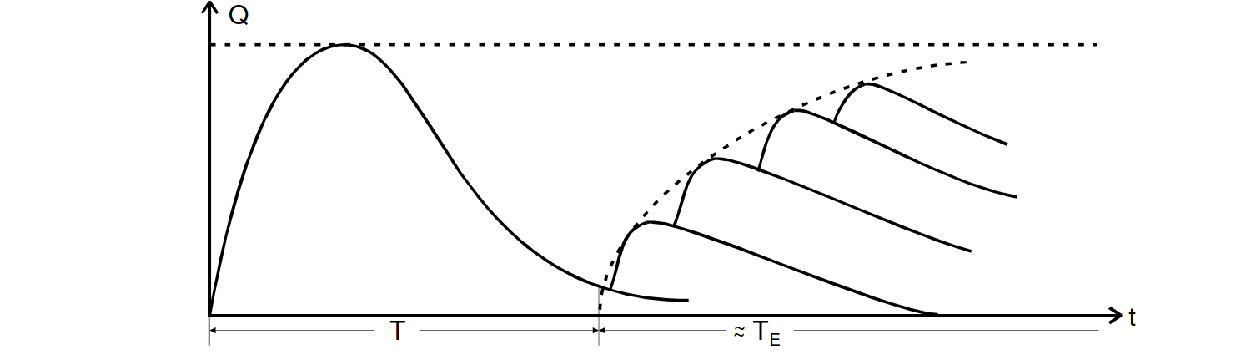
\includegraphics[width=\textwidth]{content/totzeit.pdf}
    \caption{Tot- und Erholungszeit eines Zählrohrs, dargestellt im Ladungs-Zeit-Diagramm.\cite{anleitung}}
    \label{fig:totzeit}
\end{figure}
Nach einem Entladevorgang kommt es im Zählrohr zu der Totzeit $T$ (siehe \autoref{fig:totzeit}), in dem ein neu eintretendes Teilchen nicht registriert wird.
Aufgrund der höheren Masse der positiven Ionen, sammeln sich diese um den Draht.
Dadurch wird die elektrische Feldstärke heruntergesetzt, sodass die ausgelösten Elektronen nicht mehr genug Energie für die Stoßionisation bekommen.
Daher gibt es keinen Ladungsimpuls mit dem das Teilchen registriert wird.
Mithilfe von zwei Quellen kann die Totzeit eines Zählrohrs ermittelt werden. 
Die registrierte Zählrate $N_{\text{r}}$ steht im Zusammenhang mit der Anzahl der ins Zährohr eintretenden Teilchen $N_{\text{w}}$:
\begin{equation*}
    N_{\text{w}} = \frac{N_{\text{r}}}{1-T\cdot N_{\text{r}}}
\end{equation*}
Werden die registrierten Impulsraten für zwei verschiedene Quelle, einzeln und zusammen gemessen, gilt:
\begin{equation*}
    \frac{N_{1+2}}{1-TN_{1+2}} = \frac{N_1}{1-TN_1}+\frac{N_2}{1-TN_2}
\end{equation*}
Für $T^2N_{\text{i}}^2 <<1$ gilt folgende Näherung:
\begin{equation*}
    T \approx \frac{N_1 + N_2 - N_{1+2}}{2N_1N_2}
\end{equation*}
Die Erholungszeit $T_{\text{E}}$ bezeichnet den Zeitraum, in dem neu eintreffende Teilchen registriert werden, aber die Ladungsimpulse nicht die ursprüngliche Höhe haben.
Die positiven Ionen, die sich um den Draht gesammelt haben, wandern zum Mantel ab und werden neutralisiert.
Sobald alle Ionen vollständig neutralisiert sind, haben die Ladungimpulse wieder die ursprüngliche Höhe.
In der \autoref{fig:totzeit} ist in der gestrichelten Linie die Einhüllende zu sehen.
Da diese sehr flach ist, ist die Erholungszeit $T_{\text{E}}$ praktisch nur ungenau bestimmbar.
Aus dem mittleren Zählrohrstrom 
 \begin{equation*}
     \bar{I} \coloneq \frac{1}{\tau} \int_0^{\tau} \frac{U(t)}{R}\,\symup{d}t
 \end{equation*} 
 lässt sich die Ladungsmenge pro eindringendem Teilchen berechnen.
 Außerdem gilt für die in dem Zeitintervall $\increment t$ registrierte Anzahl von Teilchen $Z$ und transportierte Ladungsmenge $\increment Q$:
 \begin{equation*}
     \bar{I} = \frac{\increment Q}{increment t} Z
 \end{equation*}\\
Bei der Neutralisierung der Ionen an dem Stahlmantel wird Energie frei, mit der wieder Elektronen ausgelöst werden können.
Diese Elektronen werden Sekundärelektronen genannt und können einen Entladungsvorgang starten.
Da die Ionen von ihrem Entstehungsort zum Stahlmantel in der Zeit $T_{\text{L}}>T$ wandern, gibt es mit pro eingetretendem Teilchen mehrere Nachentladungen.
Mit Alkoholdampf in dem Gasgemisch werden viele der Nachentladungen unterdrückt.\\
\\
Das Ansprechvermögen eines Zählrohres beschreibt die Wahrscheinlichkeit, dass ein einfallendes Teilchen registriert wird.
Für geladene Teilchen, wie $\alpha$- oder $\beta $ -Teilchen ist das Ansprechvermögen bei ca $\SI{100}{\percent}$.
Das Geiger-Müller-Zählrohr ist für Messungen hoher $\gamma$ Intesitäten benutzbar, das Ansprechvermögen für Photonen ist sehr gering.\\
Als Charakteristik eines Zählrohrs wird das $U$-$N$ Diagramm, in dem die registrierte Teilchenzahl $N$ bei konstanter Strahlungsintensität gegen die angelegte Spannung $U$ aufgetragen wird, bezeichnet.
In der \autoref{fig:charakteristik} ist do ein Diagramm zu sehen. 
Die Spannung $U_{\text{E}}$ zeigt den Beginn des Auslösebereichs an. 
Das Plateau der Kurve ist der Arbeitsbereich des Zählrohrs.
Ein ideales Zählrohr hat keine Plateausteigung, die Qualität des Zählrohrs ist an der Länge und Steigung des Plateaus abzulesen.
Dem Plateau folgt der Bereich der Dauerentladung, welches dem Bereich V in der \autoref{fig:bereiche} entspricht.
\begin{figure}
    \centering
    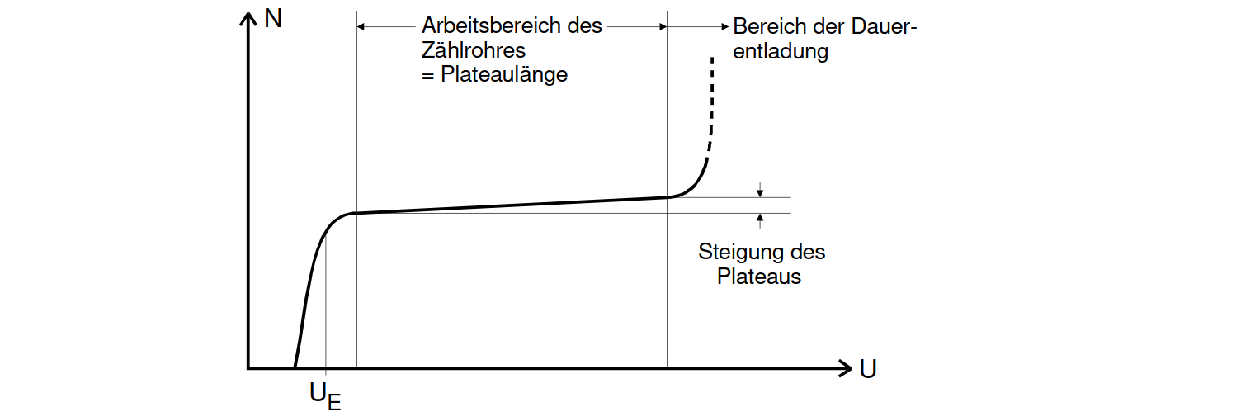
\includegraphics[width=\textwidth]{content/charakteristik.pdf}
    \caption{Zählrohrcharakteristik \cite{anleitung}}
    \label{fig:charakteristik}
\end{figure}